\documentclass[16pt]{article}
\usepackage[russian]{babel}
\usepackage{a4wide}
\usepackage[utf8]{inputenc}
\usepackage{graphicx}
\usepackage{amsmath}
\usepackage{amssymb}
\usepackage{amsthm}
\usepackage{import}
\usepackage{xifthen}
\usepackage{pdfpages}
\usepackage{transparent}
\usepackage{multicol}
\usepackage{animate}

\newcommand{\incfig}[2]{%
    \def\svgwidth{#2 mm}
    \import{./figures/}{#1.pdf_tex}
}

\newtheorem{Th}{Теорема}
\newenvironment{Proof}{\par\noindent{\bf Доказательство.}}{\hfill$\scriptstyle\blacksquare$}
\newenvironment{Sol}{\par\noindent{\it Решение:}}


\DeclareMathOperator{\Arccos}{arccos}
\DeclareMathOperator{\Arctg}{arctg}
\DeclareMathOperator{\Cl}{Cl}
\DeclareMathOperator{\Ker}{ker}
\DeclareMathOperator{\Ima}{im}
\DeclareMathOperator*{\Argmax}{Argmax}
\DeclareMathOperator*{\Var}{Var}


\newcommand\Real{\mathbb{R}} 
\newcommand\A{(\cdot)} 
\newcommand\Sup[2]{\rho( #1 \, | \, #2 )}
\newcommand\Sum[2]{\sum\limits_{#1}^{#2}}
\newcommand\Scal[2]{\langle #1,\, #2 \rangle}
\newcommand\Norm[1]{\left\| #1 \right\|}
\newcommand\Int[2]{\int\limits_{#1}^{#2}}
\newcommand\PS{\mathcal{P}}
\newcommand\X{\mathcal{X}} 
\newcommand\Pict[3]{
\begin{figure}[h!]
    \centering
    \incfig{#1}{#3}
    \caption{#2}
    \label{fig:#1}
\end{figure}
}


\begin{document}

\thispagestyle{empty}

\begin{center}
\ \vspace{-3cm}


\includegraphics[width=0.5\textwidth]{msu.eps}\\
{\scshape Московский государственный университет имени М.~В.~Ломоносова}\\
Факультет вычислительной математики и кибернетики\\
Кафедра системного анализа

\vfill

{\LARGE Отчёт по заданию 1 курсовой работы}

\vspace{1cm}

{\Huge\bfseries <<Динамические системы с дискретным временем>>}
\end{center}

\vspace{1cm}

\begin{flushright}
  \large
  \textit{Студент 315 группы}\\
  Д.\,М.~Сотников

  \vspace{5mm}

  \textit{Руководитель практикума}\\
  Д.\,А.~Алимов
\end{flushright}

\vfill

\begin{center}
Москва, 2020
\end{center}

\newpage

\section{Постановка задачи}
Даны две динамические системы с дискретным временем
\begin{equation} \label{s1}
u_{t+1} = r\sqrt{u_t}(1 - au_t^3),
\end{equation}
\begin{equation} \label{s2}
u_{t+1} = r\sqrt{u_t}(1 - au_{t-1}^3),
\end{equation}
где $r > 0, \ a > 0, \ u_t \geqslant 0 \ \ \forall t  \in \mathbb{N}.$

Для этих систем нужно
\begin{itemize}
\item
Найти неподвижные точки.
\item
Исследовать их на устойчивость.
\item
Проверить существование циклов длины 2 и 3.
\item
При наличии цикла длины 3 построить бифуркационную диаграмму.
\item
Построить график показателя Ляпунова в зависимости от значений параметра.
\item Для системы (\ref{s2}) проверить возможность возникновения бифуркации Неймарка-Сакера.
\end{itemize}

\section{Интерпретация и анализ параметров}
Система (\ref{s1}) описывает изменение численности некоторой популяции в дискретном времени. В условиях отсутствия
внутривидовой конкуренции чиленность растет как $r\sqrt{u_t}$, конкуренция же описывается функцией $(1-au_t^3)$.
 
Таким образом параметр $r$ отвечает за естественный рост популяции, параметр $a$ описывает конкуренцию.
Обозначим $f(u) = r\sqrt{u}(1-au^3)$.
Очевидно, что численность популяции неотрицательна, поэтому $(1-au_t^3) \geqslant 0 \ \forall t \in \mathbb{N}$, откуда 
$$0 \leqslant u_t \leqslant u_{max} = a^{-\frac{1}{3}} \quad \forall t \in \mathbb{N}.$$ Отсюда же имеем ограничение 
$f(u_t) \leqslant u_{max}$.
Функция $f$ достигает максиум в точке \\$u_0~=~(7a)^{-\frac13}~\in~[0,\,u_{max}]$, при этом 
$f_{max} = f(u_0) = \frac{6r}{7}(7a)^{-\frac16}$.

Из условия $f_{max} \leqslant u_{max}$ получаем $$0 < a \leqslant a_{max} = 7\left(\dfrac{7}{6r}\right)^6.$$

Для второго уравнения введем функцию $g(u, v) = r\sqrt{u}(1-av^3)$.
Система (\ref{s2}) является системой с запаздыванием, ее интерпретация абсолютно аналогична с единственным отличием:
в конкуренции участвует предыдущее поколение $u_{t-1}$. Значения $u_1,\, u_2 \in [0,\, u_{max}]$  задаются
как начальное условие. Так как для любых допустимых начальных условий требуется $g(u_1, u_2) \leqslant u_{max},$ а максимальное
значение $g$ равно $r\sqrt{u_{max}} = ra^{-\frac16}$, имеем следующее ограничение
$$0 < a \leqslant a_{max} = \frac{1}{r^6}.$$

Заметим, что график функций $f, g$ при $r = 1$ и произвольном $a \in \left[0,\,7\left(\frac{7}{6}\right)^6\right]$ совпадает с графиком при
произвольном $r > 0$ и $a_1 = \frac{a}{r^6} \in \left[0,\,7\left(\frac{7}{6r}\right)^6\right]$ с точностью
до растяжения в $r^2$ раз. Это следует из того, что при таких значениях параметров
$$f(r^2u) = r^2f(u).$$
Для функции $g$ этот эффект рассматривается аналогично.
Таким образом в этих случаях фазовые портреты системы будут предсталять собой одну и ту же топологическую сущность,
поэтому достаточно рассмотреть случай $r = 1$.
Окончательно имеем
\begin{equation} \tag{\ref{s1}$'$} \label{ss1}
u_{t+1} = f(u_t) = \sqrt{u_t}(1 - au_t^3),
\end{equation} 
\begin{equation} \tag{\ref{s2}$'$} \label{ss2}
u_{t+1} = g(u_t, u_{t-1}) = \sqrt{u_t}(1 - au_{t-1}^3),
\end{equation}
$$u_t \in [0,\, u_{max}],\quad u_{max} = a^{-\frac{1}{3}}.$$
Для первой системы $$0 < a \leqslant a_{max} = 7\left(\dfrac{7}{6}\right)^6 \approx 17.65.$$
Для второй $$0 < a \leqslant 1.$$

\section{Анализ системы 1}
\subsection{Неподвижные точки}
Неподвижные точки обоих систем совпадают и удовлетворяют уравнению
$$u = \sqrt{u}(1 - au^3).$$

Одно из решений --- точка $u = 0$. Эта неподвижная точка является неустойчивой, поскольку вблизи нуля функция $f$
эквивалентна $\sqrt{u}$, и, как видно из диаграммы Ламерея, $u$ будет отдаляться от нуля.
\Pict{root}{Неустойчивость точки $u = 0$.}{70}

Нетривиальное положение равновесия удовлетворяет уравению
$$\sqrt{u} = (1 - au^3).$$
Так как функция $h(u) = 1 - au^3 - \sqrt{u}$ имеет на концах отрезка $[0,\, u_{max}]$ разные знаки, то
это уравнение имеет решение $u^*$, а так как $h'(u) = -3au^2 - \frac{1}{2\sqrt{u}} < 0$, это решение единственно.
%
%\begin{figure}[h]
%\noindent\centering{
%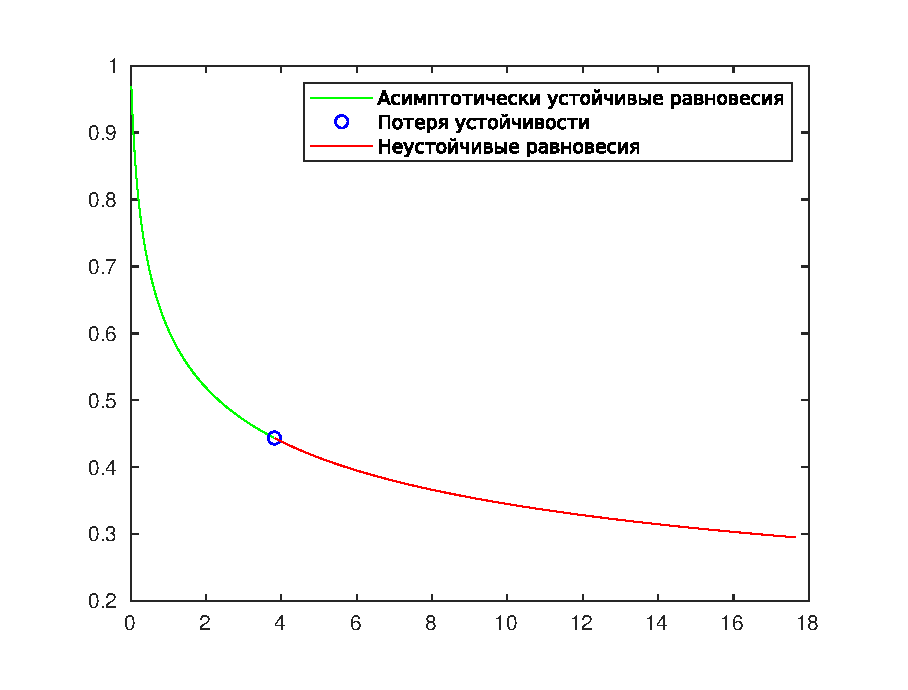
\includegraphics[width=120mm]{equils.eps}
%}
%\caption{Зависимость $u^*$ от $a$.}
%\label{figCurves}
%\end{figure}
%\newpage
Устойчивость $u^*$ зависит от значения $f'_u = \dfrac{1-7au^3}{2\sqrt{u}}$ в этой точке. Находя численно значения
$u^*$ и подставляя их в $f'_u$, можно сделать вывод, что $u^*$ асимптотически устойчива при $0 < a < a_0$ и
неустойчива при $a_0 < a < a_{max}$. Значение $a_0$ примерно равно $3.8127$. Ниже приведены иллюстрации численных
расчетов.
\newpage

\begin{center}
\begin{figure}[h]
\center
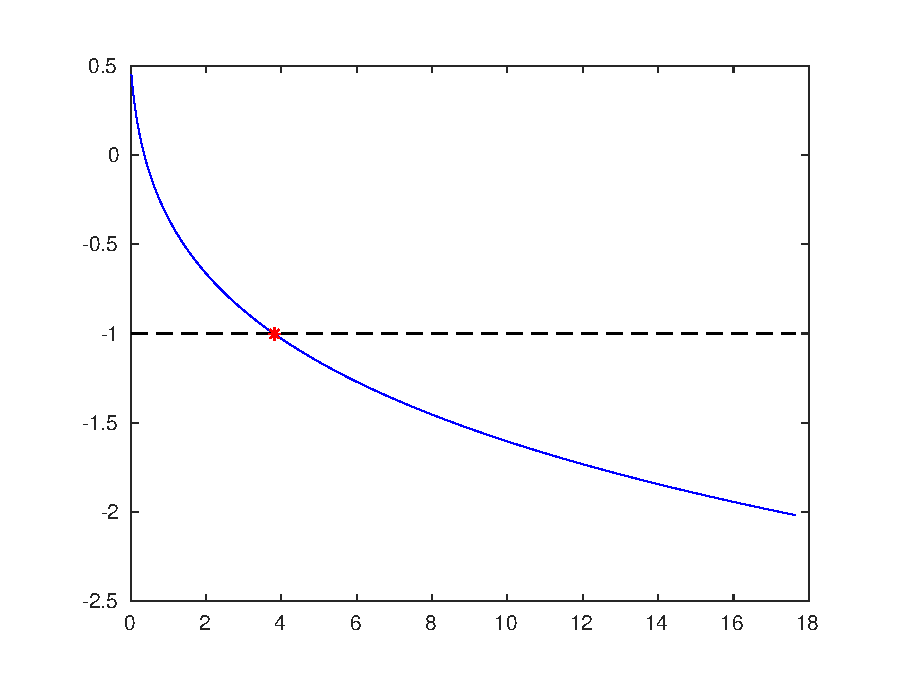
\includegraphics[width=100mm]{der.eps}
\caption{Значения $f'_u(u^*)$.}
\end{figure}
\begin{figure}[h]
\center
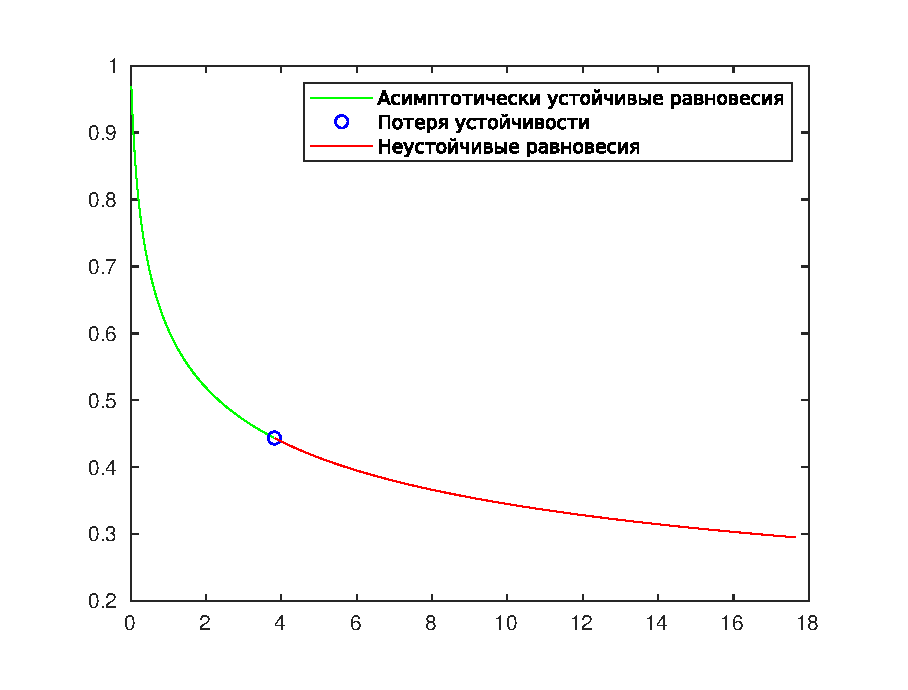
\includegraphics[width=100mm]{equils.eps}
\caption{Устойчивость неподвижной точки.}
\end{figure}

\end{center}
%\flushleft

\newpage
\subsection{Возникновение циклов}
\begin{figure}[h]
\begin{multicols}{2}
	\hfill
	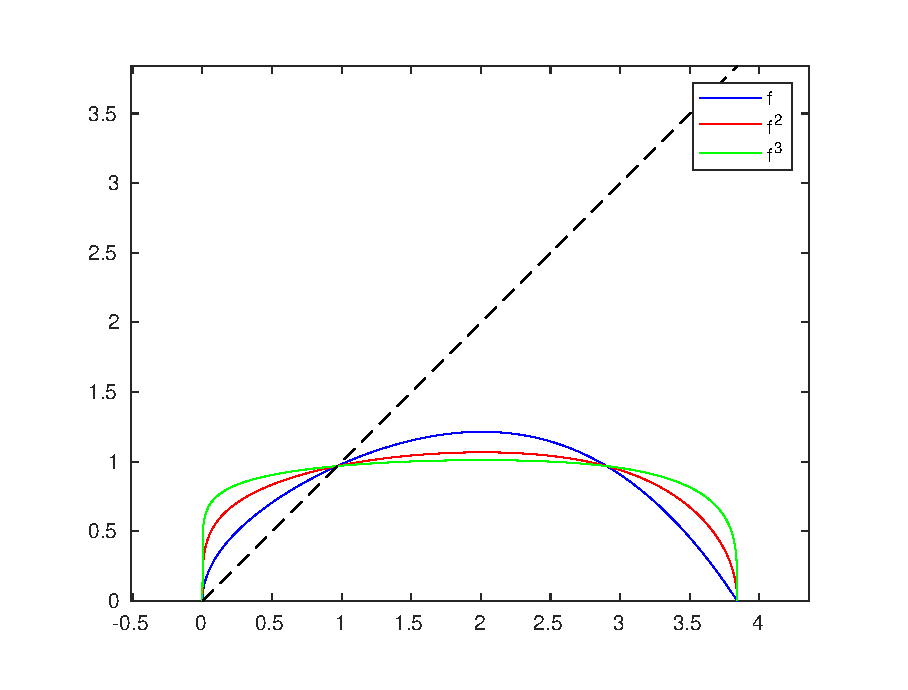
\includegraphics[width=80mm]{f1.eps}
	\hfill
	\caption{$a = 0.001$.}
	\hfill
	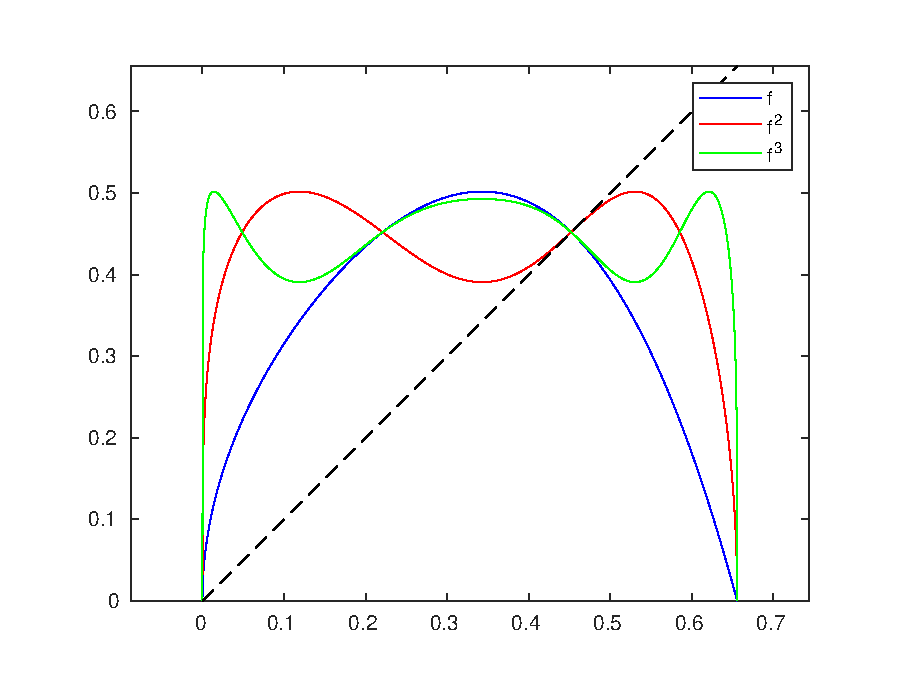
\includegraphics[width=80mm]{f2.eps}
	\hfill
	\caption{$a = 0.2a_{max}.$}
    \hfill
\end{multicols}

\begin{multicols}{2}
	\hfill
	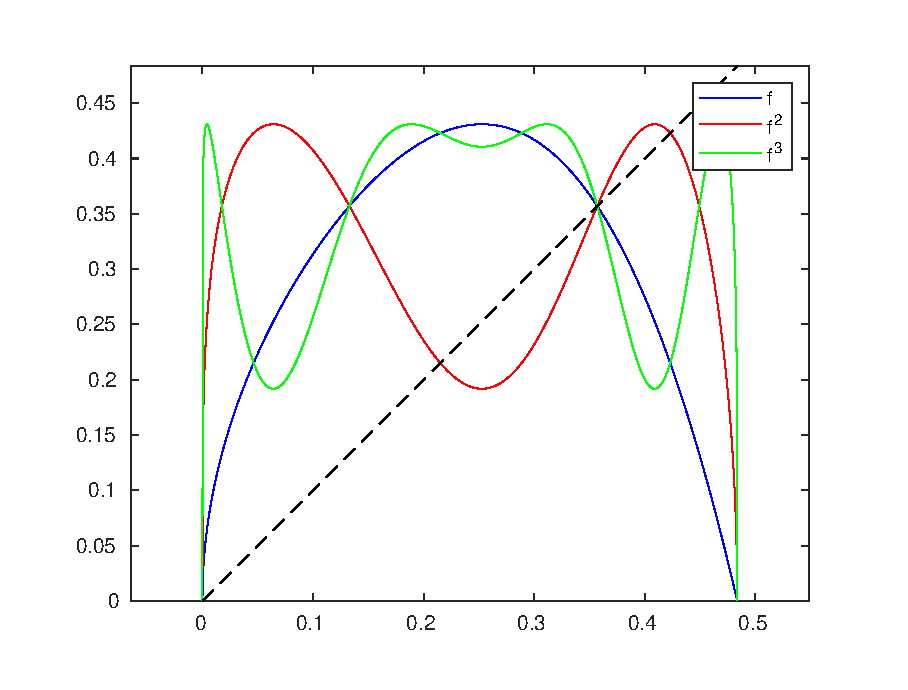
\includegraphics[width=80mm]{f3.eps}
	\hfill
	\caption{$a = 0.5a_{max}$.}
	\hfill
	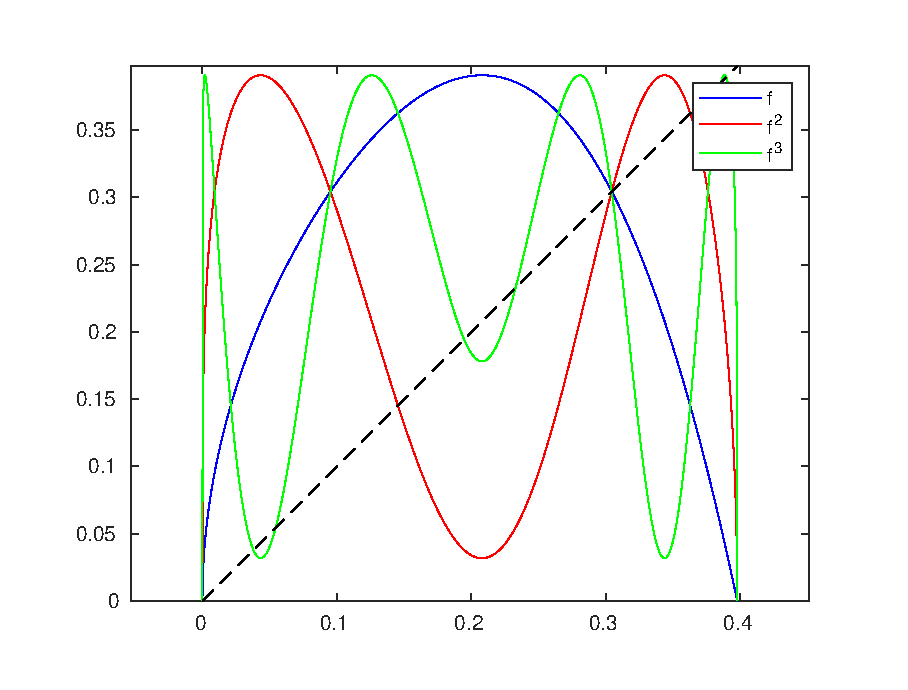
\includegraphics[width=80mm]{f4.eps}
	\hfill
	\caption{$a = 0.9a_{max}$.}
    \hfill
\end{multicols}
\end{figure}	

На данной иллюстрации приведены графики $f$, $f^2 = f \circ f$, $f^3 = f \circ f \circ f$, пересечения которых
с прямой $y = u$ являются неподвижными точками, элементами циклов длины 2 и элементами циклов длины 3 
соответственно. Видно, что по мере увеличения параметра $a$ сначала появляется цикл длины 2, затем
добавляются два цикла длины 3.

Построим бифуркационную диаграмму системы: при каждом значении параметра $a$ выпустим траекторию из
$0.1u_{max}$, вычислим 100 итераций для стабилизации системы, затем
следующие 100 итераций отложим на диаграмме по оси ординат.
\newpage

\begin{figure}[h]
\begin{center}
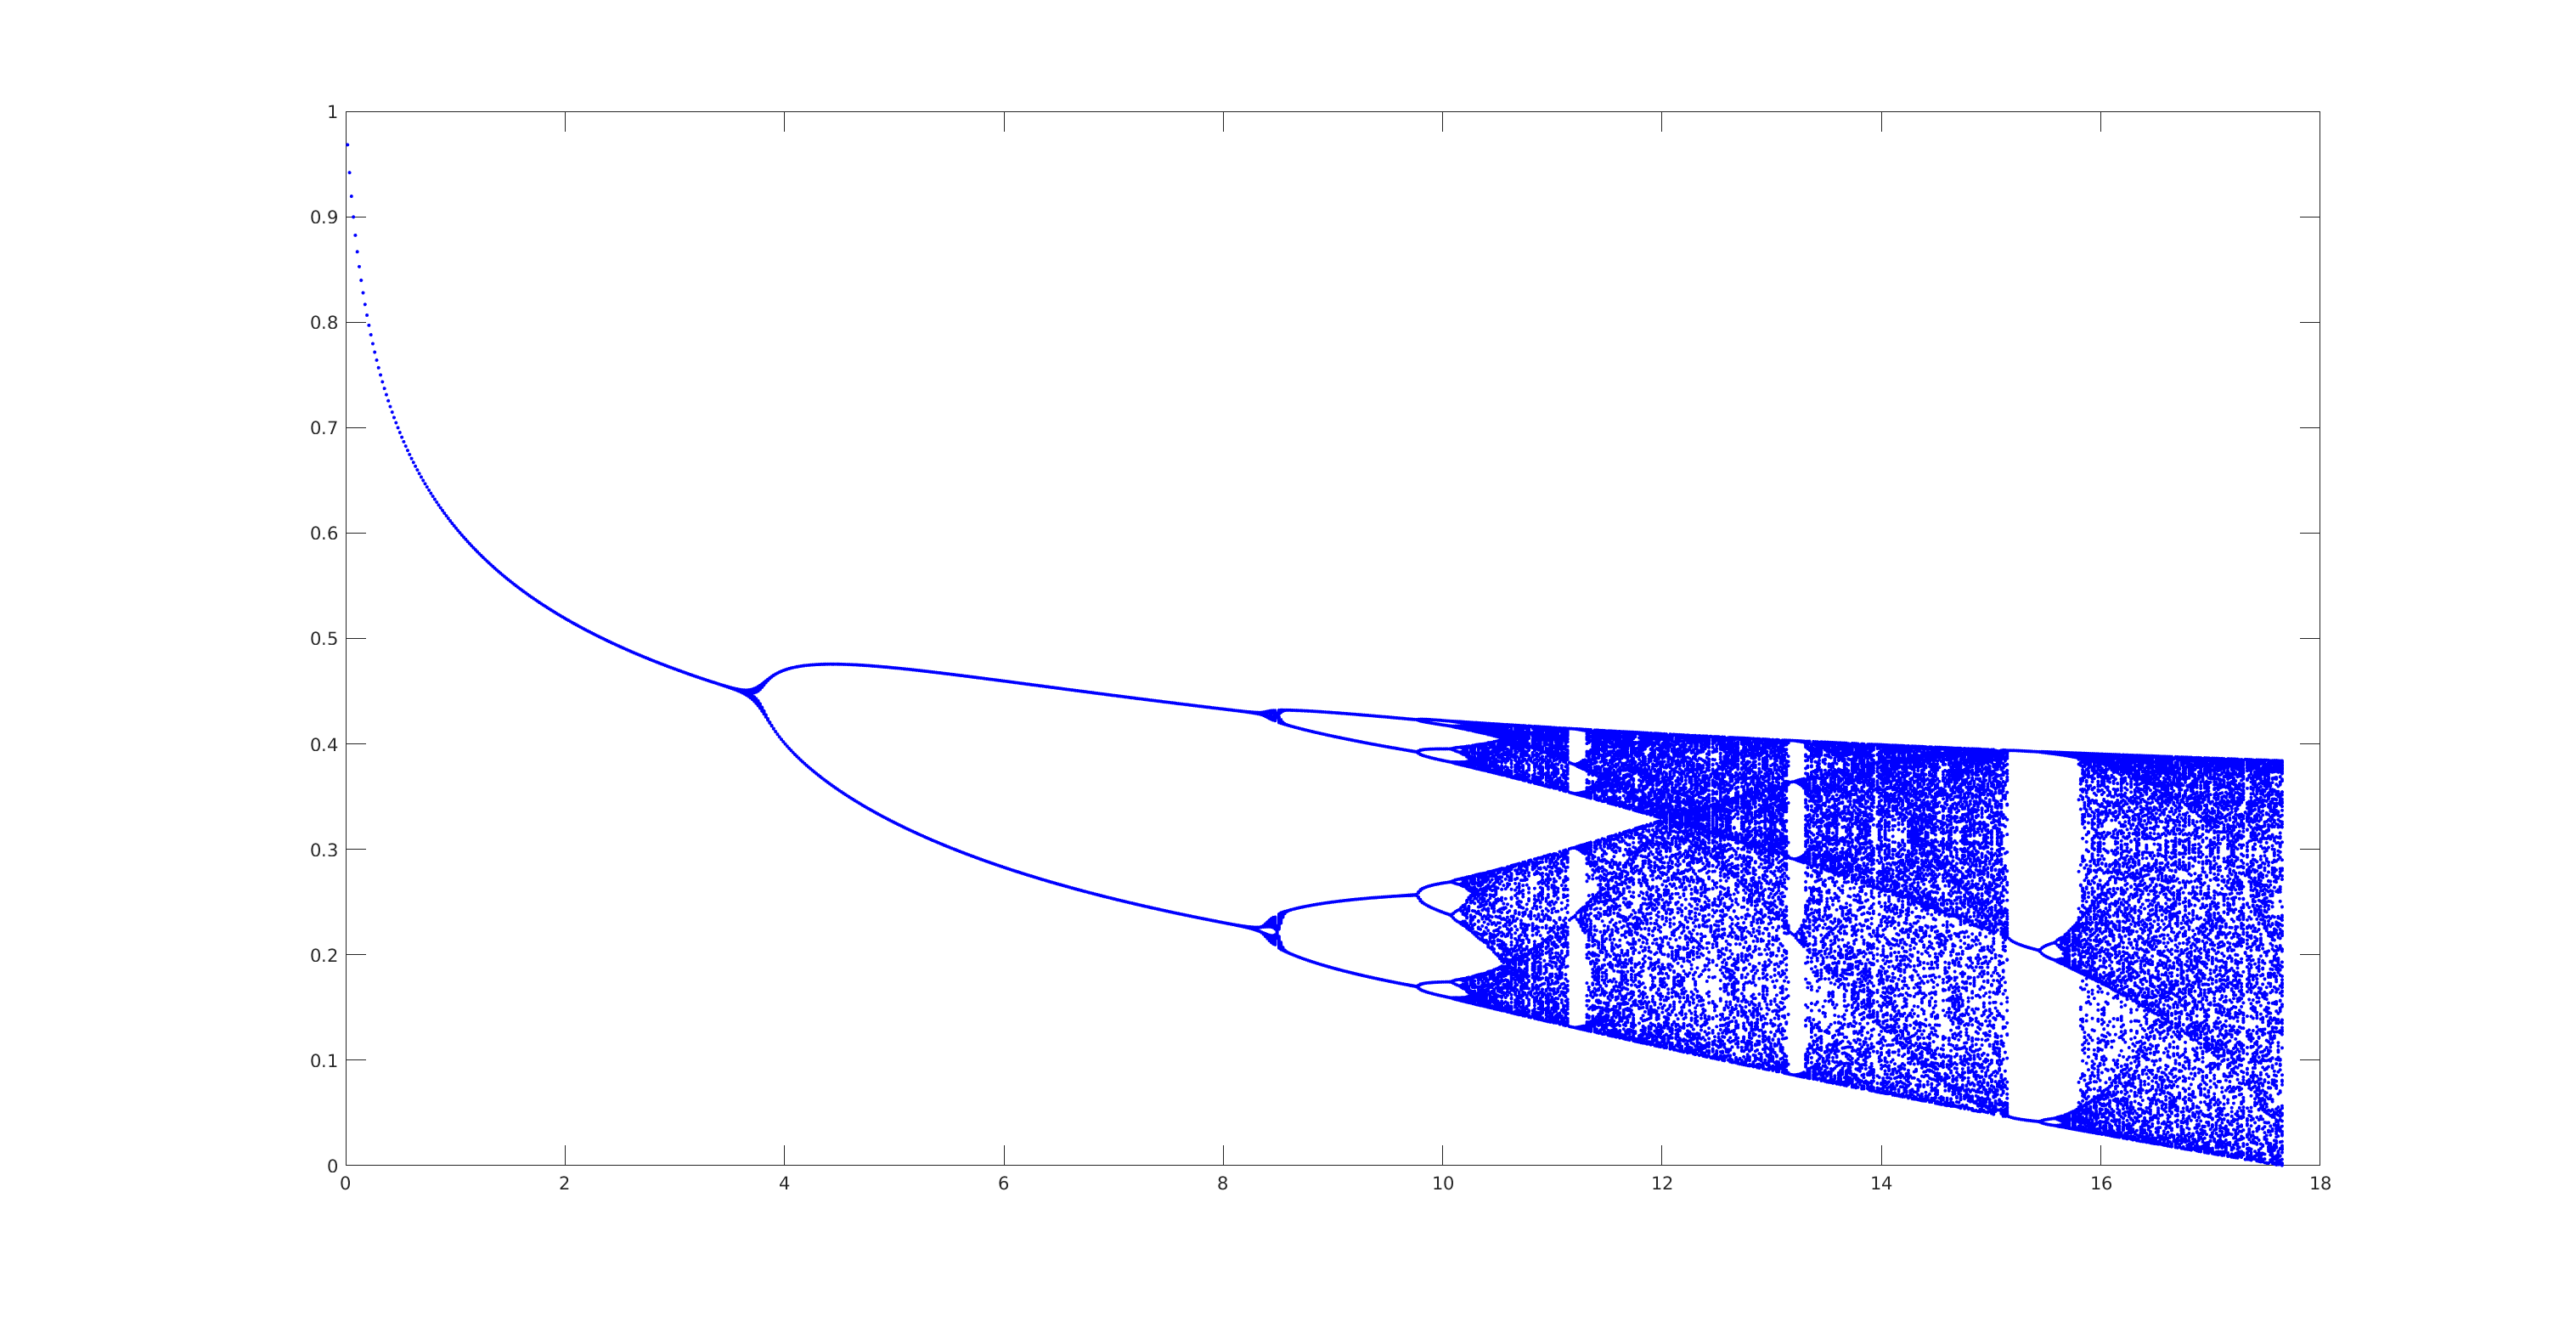
\includegraphics[width=140mm]{bif.eps} \label{bif}
\caption{Бифуркационная диаграмма при $a \in [0,\,a_{max}]$.}
\end{center}
\end{figure}

До момента $a_0$ неподвижная точка является глобально устойчивой, затем при $a = a_1$ устойчивость теоряется 
и появляется
устойчивый цикл длины 2. При более детальном рассмотрении диаграммы на сегменте $[15,\,16]$ обнаруживается
устойчивый цикл длины 3. 

\begin{figure}[h]
\begin{center}
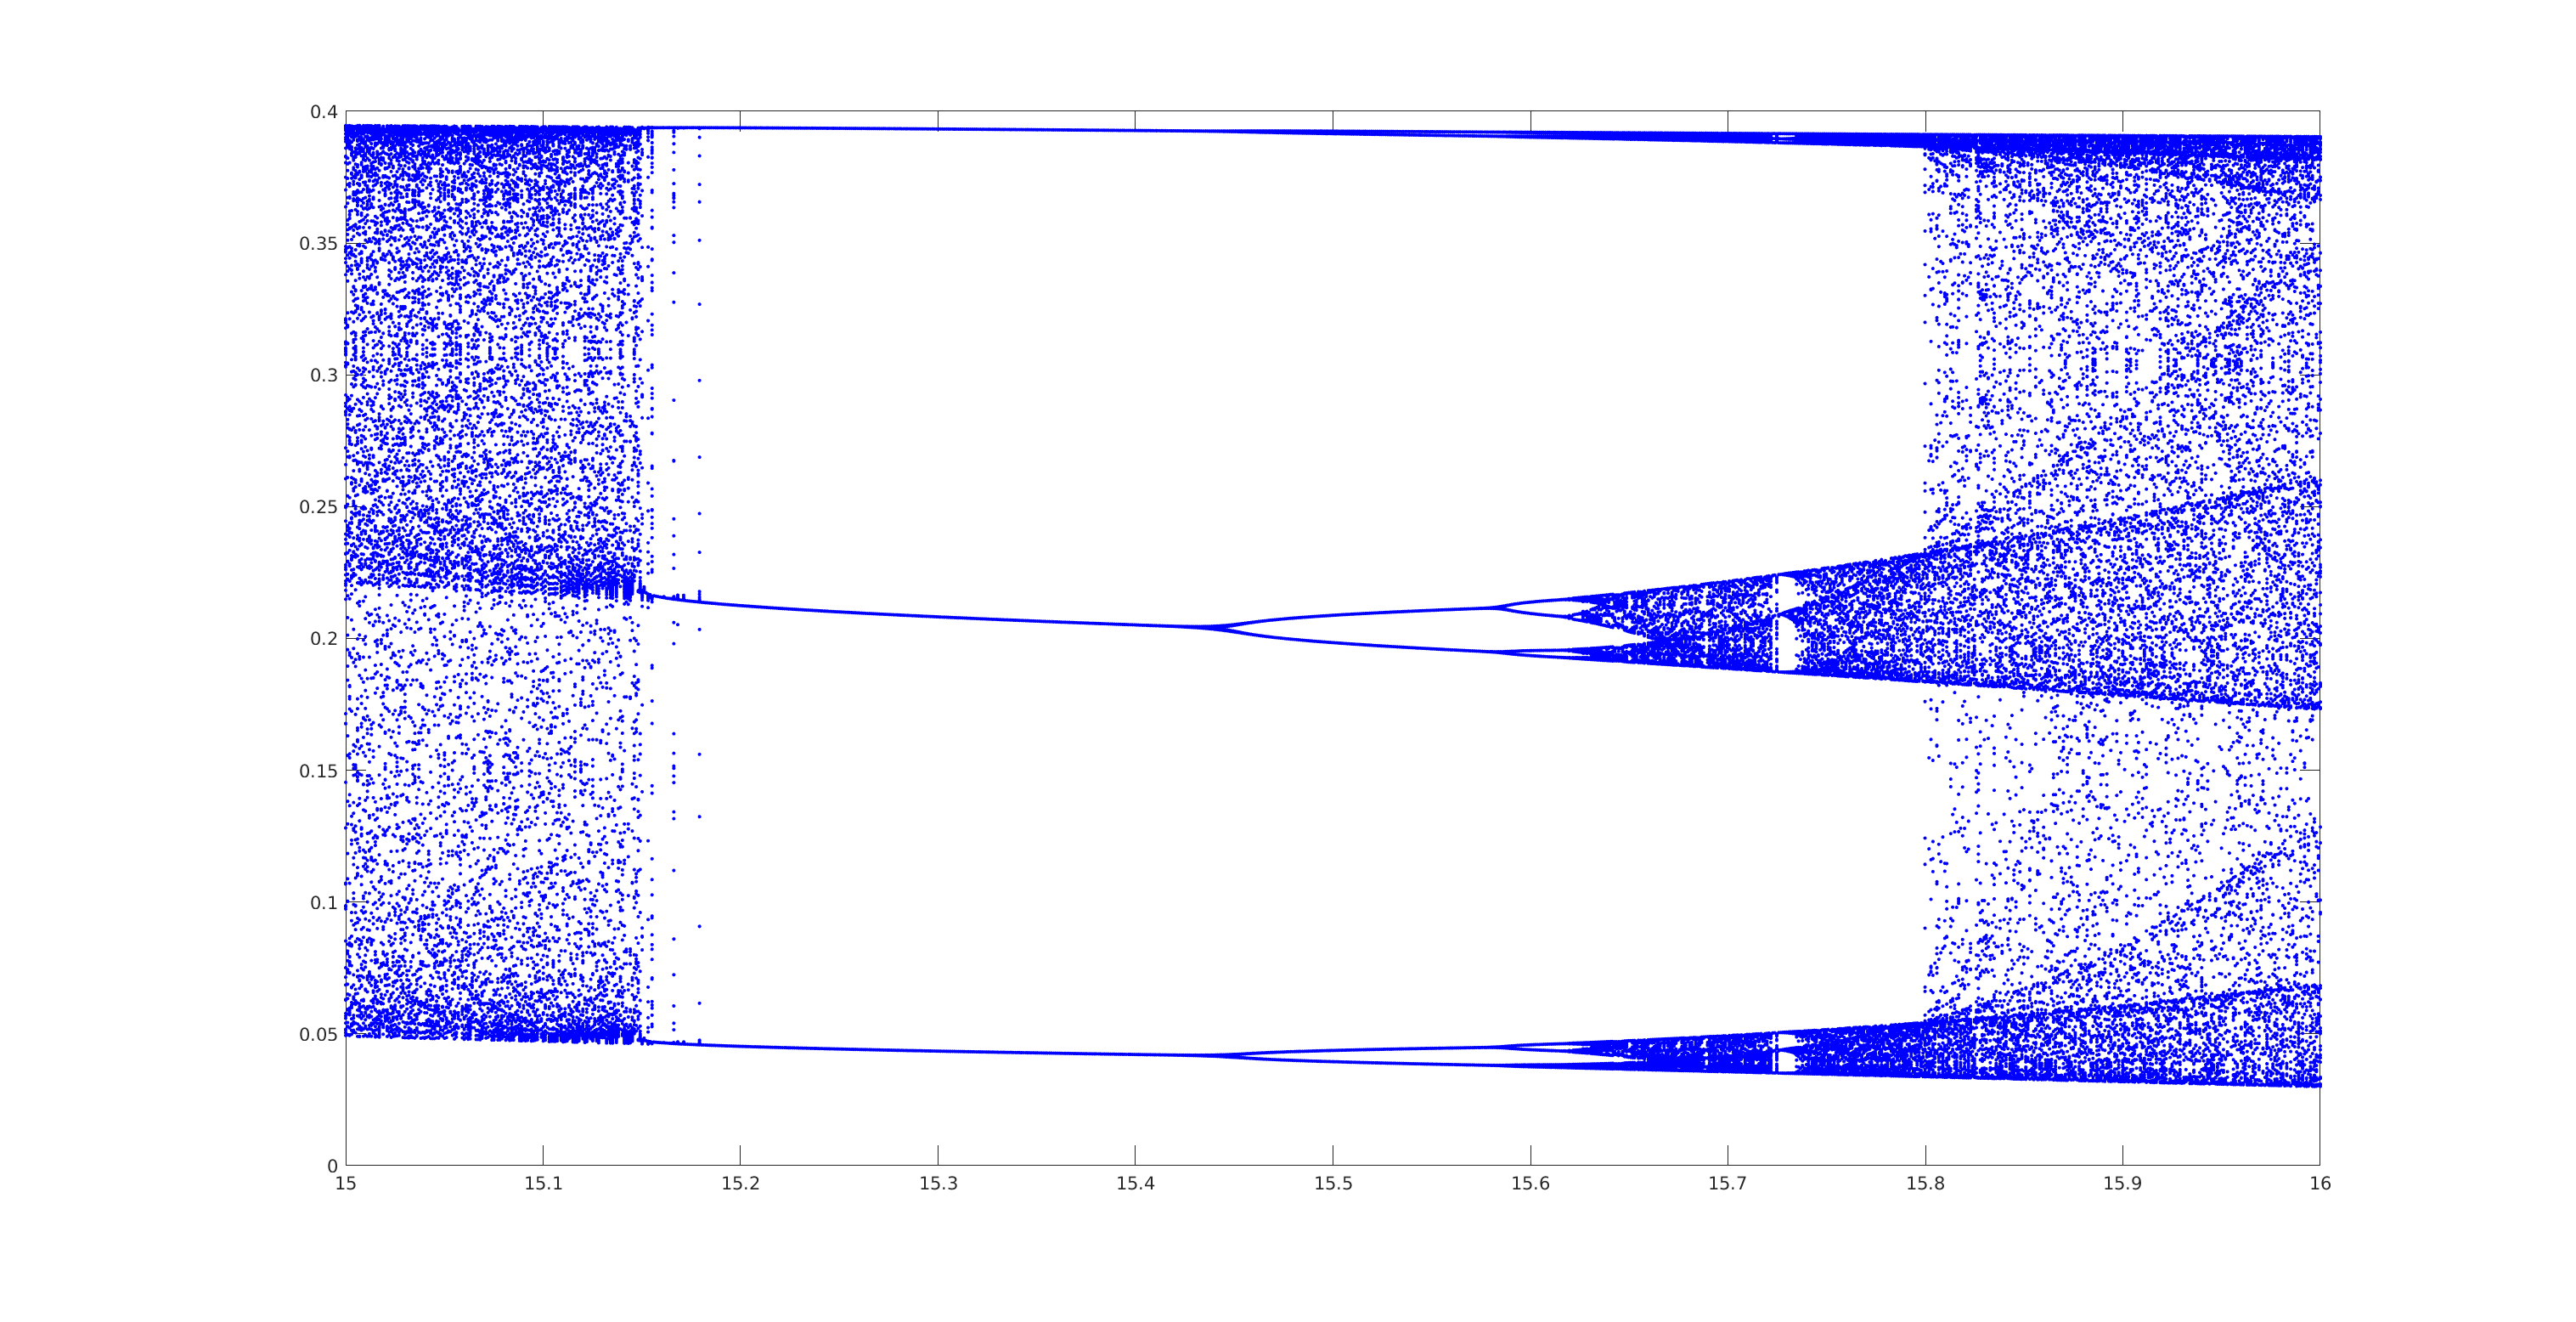
\includegraphics[width=140mm]{bif2.eps} \label{bif2}
\caption{Бифуркационная диаграмма при $a \in [15,\, 16]$.}
\end{center}
\end{figure}
%\begin{center}
%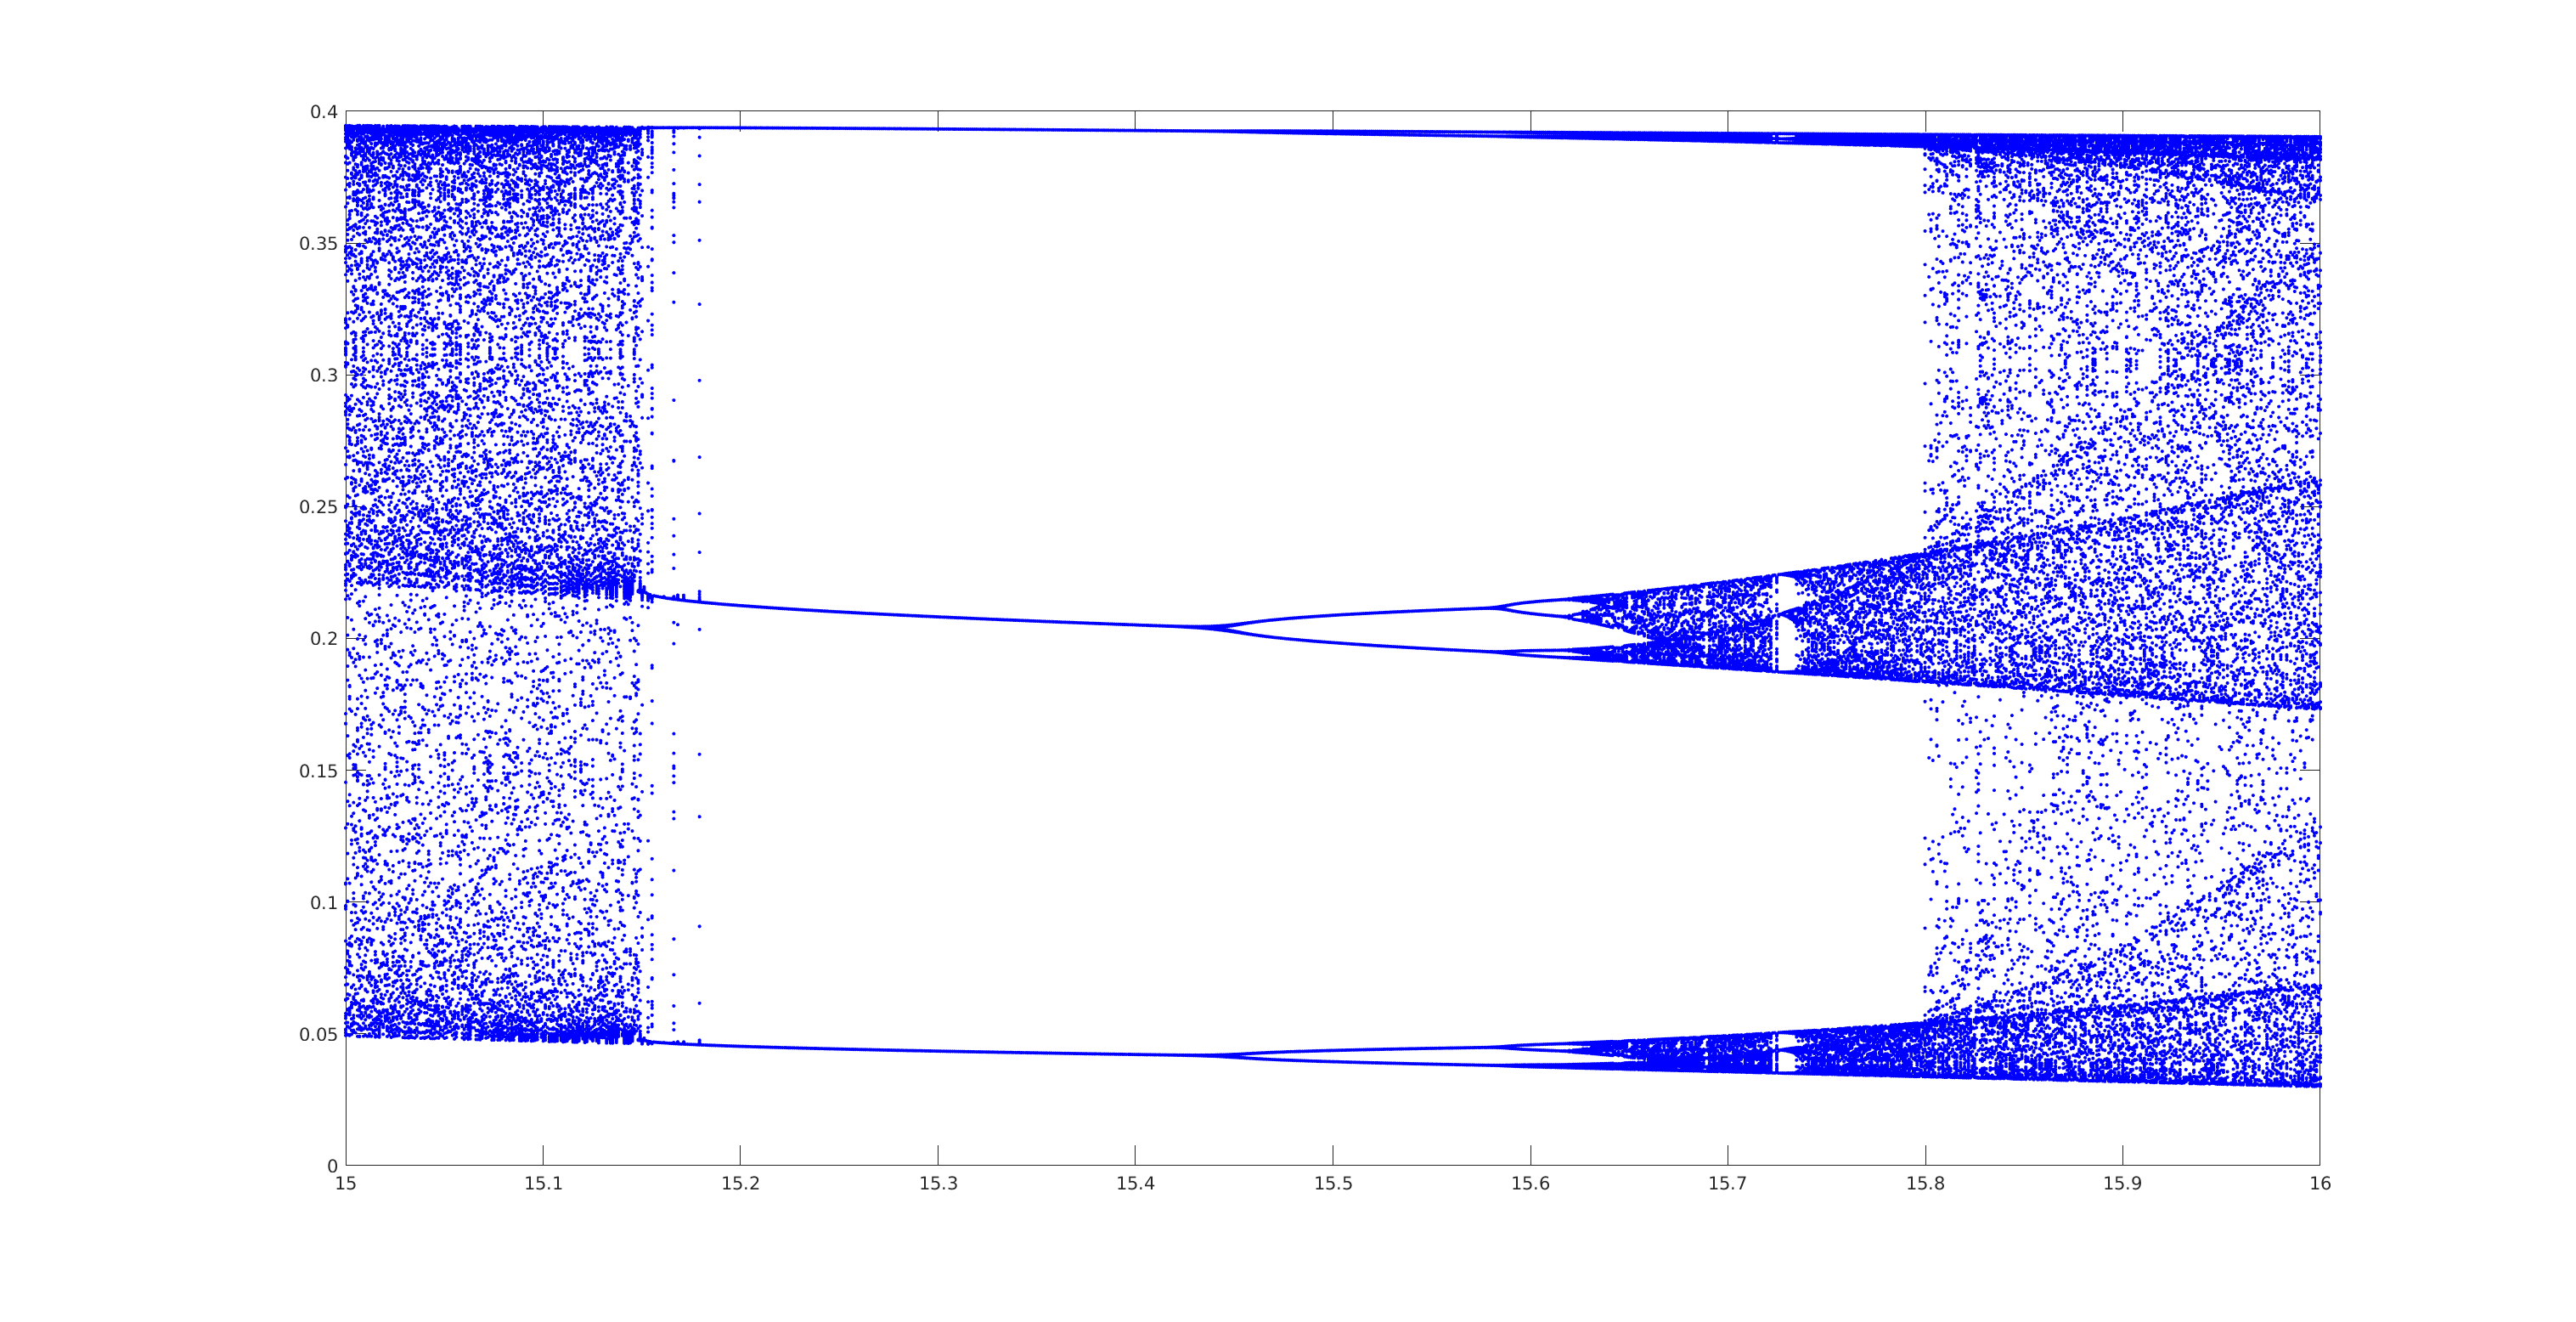
\includegraphics[width=160mm]{bif2.eps}
%\end{center}

\newpage
Найдем эти циклы при параметрах $a = 6$ и $a = 15.3$.

\begin{figure}[h]
\begin{center}
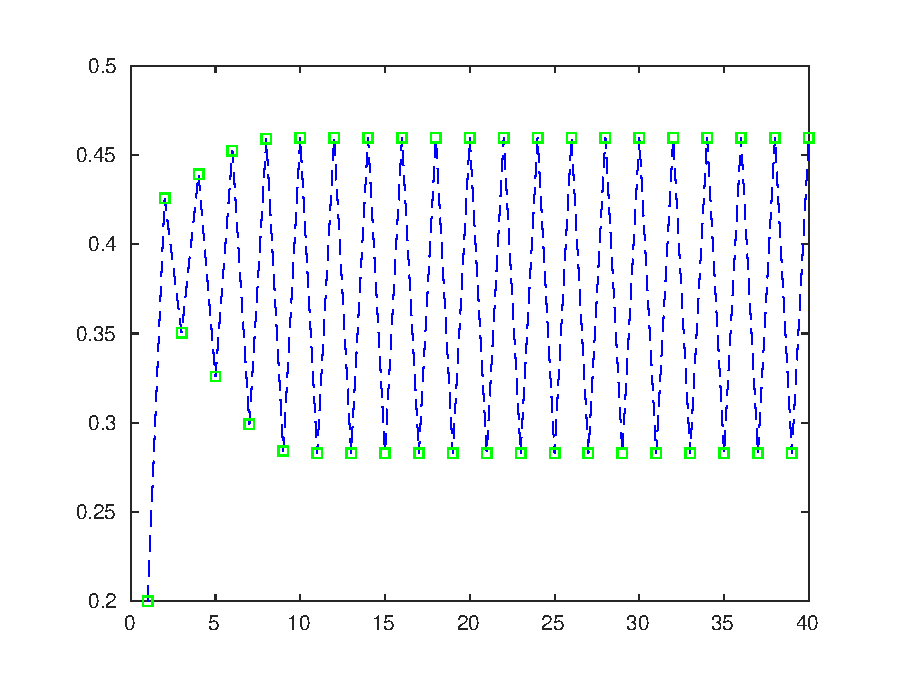
\includegraphics[width=95mm]{cycle2.eps}
\caption{Устойчивый цикл длины 2.}
\end{center}
\end{figure}
%\flushleft

Численно находятся точки цикла $u_1 \approx 0.283, \ u_2 \approx 0.4596$.

\begin{figure}[h]
\begin{center}
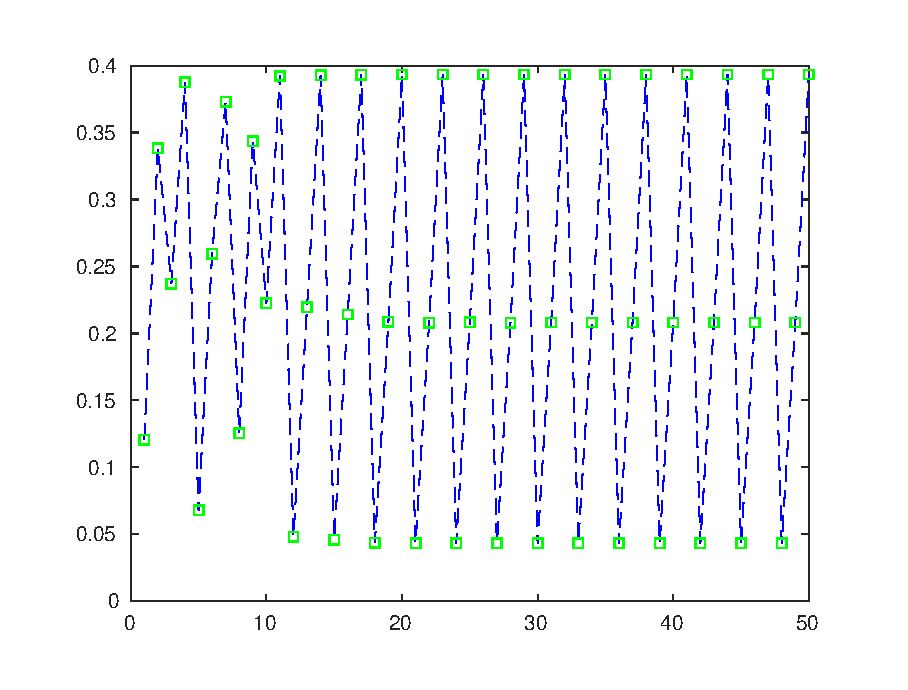
\includegraphics[width=95mm]{cycle3.eps}
\caption{Устойчивый цикл длины 3.}
\end{center}
\end{figure}

%\flushleft

Аналогично находим точки $u_1 \approx 0.0435,\ u_2 \approx 0.2082, \ u_3 \approx 0.3933$ для цикла длины 3.

\newpage
\subsection{Показатель Ляпунова}
Показатель Ляпунова для траектории --- величина, равная
$$h(u) = \lim_{n \to \infty} \dfrac{\ln|f'(u_1)| + \ln|f'(u_2)| + \ldots + \ln|f'(u_n)|}{n},$$
является мерой хаотичности системы: при отрицательных значениях $h$ близкие траектории приближаются друг другу,
при положительных --- разбегаются, несмотря на сколь угодно малое отклонение в начальный момент. При фиксированном
значении параметра показатели Ляпунова для разных начальных условий отличаются незначительно, поэтому можно
построить зависимость $h(u)$ от $a$, где траектрия $u$ выпускается из $0.1u_{max}$.

\begin{figure}[h]
\begin{center}
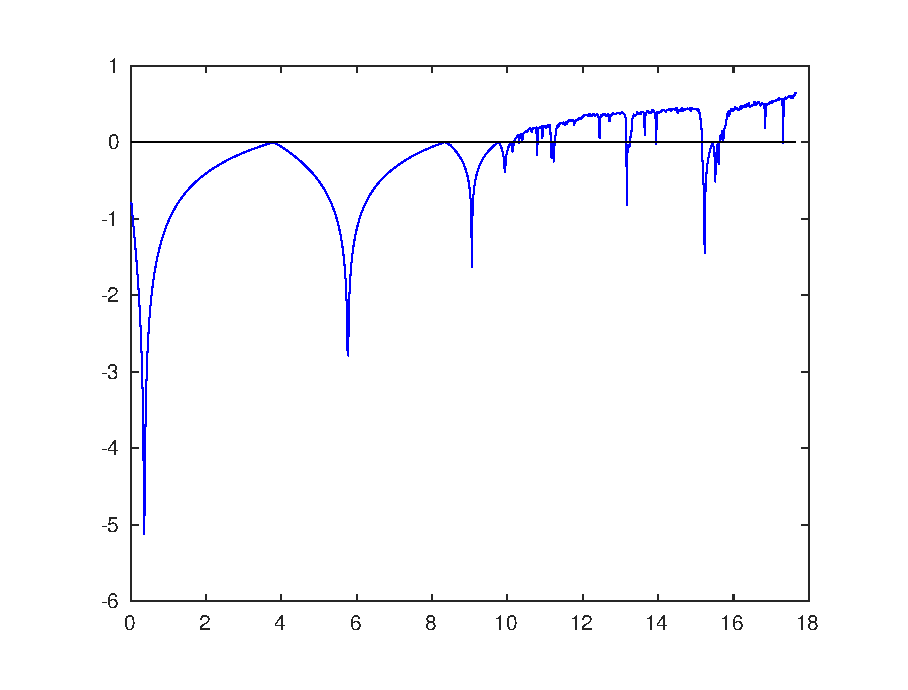
\includegraphics[width=150mm]{lyap.eps}
\caption{График показателя Ляпунова.}
\end{center}
\end{figure}

Из графика видно, что при малых значениях параметра $a$ показатель Ляпунова отрицателен, что соответствует
<<устойчивым>> состояниям системы, как, например, $a = 6$, при котором возникал устойчивый цикл длины 2.
Отметим также, что при $a \approx 15$ показатель Ляпунова отрицателен, и именно в этой полосе значений
на бифуркационной диаграмме исчезало хаотическое поведение и появлялся устойчивый цикл. Нули показателя Ляпунова соответствуют точкам
бифуркации на диаграмме. При значениях $a$, на которых показатель Ляпунова положителен,
в системе возникает хаос.

\newpage
\section{Анализ системы 2}

Система
$$u_{t+1} = g(u_t, u_{t-1}) = \sqrt{u_t}(1 - au_{t-1}^3),$$
как говорилось ранее, является системой с запаздыванием и эквивалентна следующей двумерной системе:
\begin{equation} \label{2dsys}
\begin{cases}
u_{t+1} = g(u_t, v_t)\\
v_{t+1} = u_t
\end{cases}
\end{equation}

\subsection{Неподвижные точки}
Неподвижными точками системы являются $u = 0$ и $u = u*$ --- неподвижные точки системы 1. Неустойчивость $u = 0$ 
доказывается аналогично случаю одномерной системы. Для исследования устойчивости $u = u^*$ найдем собственные
значения матрицы 
$$A = \begin{bmatrix} a_0 & a_1 \\ 1 & 0 \end{bmatrix},$$
где
$$a_0 = \dfrac{\partial g(u,v)}{\partial u}\bigg|_{(u^*,u^*)}, \quad a_1 = \dfrac{\partial g(u,v)}{\partial v}\bigg|_{(u^*,u^*)}.$$

Легко вычисляется $a_0 = \frac12, \ a_1 = -3a(u^*)^{5/2}$, и матрица
$$A = \begin{bmatrix} \frac12 & -3a(u^*)^{5/2} \\ 1 & 0 \end{bmatrix}.$$

Характеристический многочлен матрицы имеет вид
$$\lambda^2 -\frac{\lambda}{2} + 3a(u^*)^{5/2}.$$

Отсюда собственные значения матрицы равны
$$\lambda_{1,2} = \frac{1}{4} \pm \frac{1}{2}\sqrt{\frac{1}{4} - 12a(u^*)^{5/2}}.$$

Поскольку $u^*$ не вычисляется аналитически, найдем численно зависимость $|\lambda_{1,2}|$ от $a$.

\begin{figure}[h]
\begin{center}
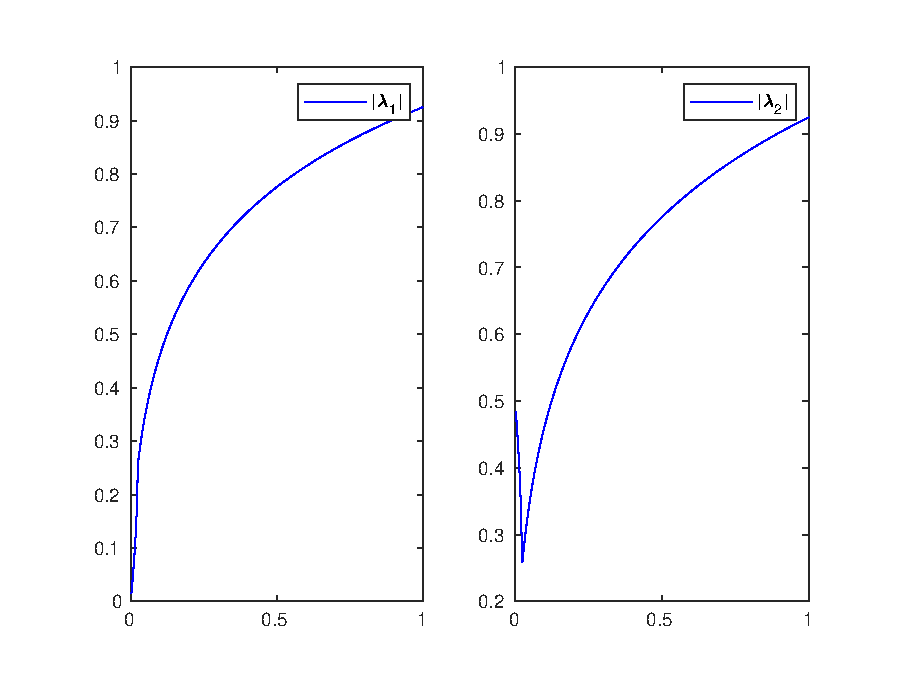
\includegraphics[width=70mm]{lambd.eps}
\caption{График $|\lambda_{1,2}|$.}
\end{center}
\end{figure}

Из графика видно, что всюду на допустимом множестве значений $a$ выполнено условие асимптотической устойчивости
$$|\lambda_i| < 1, \quad i = 1, 2.$$

Итак, точка $u = 0$ является неустойчивым положением равновесия, $u = u^*$ асимтотически устойчива при 
любых $a \in [0,\,1]$.

\subsection{Существование циклов}

Покажем, что циклов длины 2 в системе не существует. Действительно, пусть $u, v$ образуют цикл длины 2.
Тогда они удовлетворяют условию

\[
\begin{cases}
v = g(u, v) = \sqrt{u}(1-av^3)\\
u = g(v, u) = \sqrt{v}(1-au^3)
\end{cases}
\]
Деля одно уравнение на другое и разделяя переменные, получим
$$ \dfrac{u^{\frac32}}{1-au^3} = \dfrac{v^{\frac32}}{1-av^3},$$
что эквивалентно уравнению $w(x) = w(y), \ x \not= y$, где $w(x) = \frac{x}{1-ax^2}$ при $x,\ y \in [0, a^{-\frac12})$.
Но это невозможно, поскольку $w'(x) = \frac{1+ax^2}{1-ax^2} > 0$, и $w$ строго возрастает на этом сегменте.

Аналитическая проверка циклов длины 3 затруднительна, однако из асимптотической устойчивости точки и из
бифуркационной диаграммы можно предположить, что точка $u = u^*$ глобально устойчива, поэтому циклов длины 3.
система, скорее всего, иметь так же не будет.

\begin{figure}[h]
\center
\includegraphics[width=110mm]{2bif.eps}
\caption{Бифуркационная диаграмма системы}
\end{figure}

\newpage
\subsection{Бифуркация Неймарка-Сакера}
При анализе устойчивости системы было показано, что собственные значения матрицы
$$A = \begin{bmatrix} a_0 & a_1 \\ 1 & 0 \end{bmatrix}$$
не превосходят по модулю единицу при любых допустимых $a$. Отсюда можно сделать вывод, что возникновение
бифуркации Неймарка-Сакера в данной системе невозможно.
\newpage
\begin{thebibliography}{0}
\bibitem{bratus}
	Братусь~А.С., Новожилов~А.С., Платонов~А.П. Динамические системы и модели биологии. М.: ФИЗМАТЛИТ, 2010. 
\end{thebibliography}


\end{document}